% Author: Izaak Neutelings (Februari, 2020)

\documentclass[border=3pt,tikz]{standalone}
\usepackage{amsmath} % for \dfrac
\usepackage{bm}
\usepackage{physics}
\usepackage{tikz,pgfplots}
\usepackage[outline]{contour} % glow around text
\usetikzlibrary{angles,quotes} % for pic (angle labels)
\usetikzlibrary{decorations.markings}
\usetikzlibrary{calc}
\tikzset{>=latex} % for LaTeX arrow head
\contourlength{1.4pt}

\usepackage{xcolor}
\colorlet{Ecol}{orange!90!black}
\colorlet{EcolFL}{orange!90!black}
\colorlet{EFcol}{red!60!black}
\colorlet{Bcol}{violet!90}
\colorlet{BcolFL}{violet!90}
\colorlet{veccol}{green!45!black}
\colorlet{pluscol}{red!60!black}
\colorlet{minuscol}{blue!60!black}
\tikzstyle{anode}=[top color=red!20,bottom color=red!50,shading angle=20]
\tikzstyle{cathode}=[top color=blue!20,bottom color=blue!40,shading angle=20]
\tikzstyle{charge+}=[very thin,top color=red!80,bottom color=red!80!black,shading angle=-5,circle,inner sep=0.2,draw=black]
\tikzstyle{charge-}=[very thin,top color=blue!50,bottom color=blue!70!white!90!black,shading angle=10,circle,inner sep=0.2,draw=black]
\tikzstyle{vector}=[->,thick,veccol]
\tikzstyle{normalvec}=[->,thick,blue!80!black!80]
\tikzstyle{Cstyle}=[very thick,orange!90!black]
\tikzstyle{EField}=[->,thick,Ecol]
\tikzstyle{EField dashed}=[dashed,Ecol,line width=0.6]
\tikzset{
  EFieldLine/.style={thick,EcolFL,decoration={markings,
                     mark=at position #1 with {\arrow{latex}}},
                     postaction={decorate}},
  EFieldLine/.default=0.5,
  pics/Bin/.style={
    code={
      \def\R{0.12}
      \draw[pic actions,#1,line width=0.6] % ,thick
        (0,0) circle (\R) (-135:.7*\R) -- (45:.7*\R) (-45:.7*\R) -- (135:.7*\R);
  }},
  pics/Bout/.style={
    code={
      \def\R{0.12}
      \draw[pic actions,#1,fill=white,line width=0.6] (0,0) circle (\R);
      \fill[pic actions,#1] (0,0) circle (0.3*\R);
  }},
  pics/Bout/.default=Bcol,
  pics/Bin/.default=Bcol,
}
\tikzstyle{measure}=[fill=white,midway,outer sep=2]

\begin{document}


% VELOCITY SELECTOR
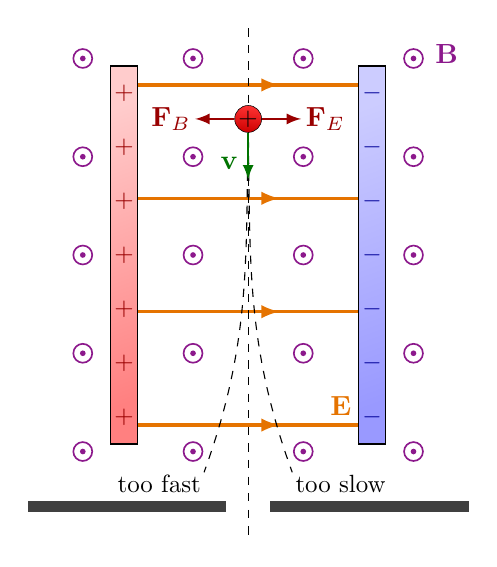
\begin{tikzpicture}
  \def\H{4.8}
  \def\W{2.8}
  \def\w{0.35}
  \def\a{0.15*\W}
  \def\NE{4}
  \def\NQ{7}
  \def\NBx{4}
  \def\NBy{5}
  
  % ELECTRIC FIELD
  \foreach \i [evaluate={\y=0.05*\H+(\i-1)*(0.9*\H)/(\NE-1);}] in {1,...,\NE}{
    \draw[EFieldLine={0.64},very thick] (0,\y) --++ (\W,0);
  }
  
  % MAGNETIC FIELD
  \foreach \i [evaluate={\y=-0.02*\H+(\i-1)*(1.04*\H)/(\NBy-1);}] in {1,...,\NBy}{
    \foreach \j [evaluate={\x=-0.25*\W+(\j-1)*(1.5*\W)/(\NBx-1);}] in {1,...,\NBx}{
      \pic[rotate=-90] at (\x,\y) {Bout};
    }
  }
  
  % PLATES
  \draw[anode]
    (0,0) rectangle++ (-\w,\H);
  \draw[cathode]
    (\W,0) rectangle++ (\w,\H);
  \foreach \i [evaluate={\y=(\i-0.5)*\H/\NQ;}] in {1,...,\NQ}{
    \node[pluscol,scale=0.9] at (-\w/2,\y) {$+$};
    \node[minuscol,scale=0.9] at (\W+\w/2,\y) {$-$};
  }
  \node[Ecol,above] at (0.92*\W,0.05*\H) {$\vb{E}$};
  \node[Bcol,above] at (1.4*\W,0.98*\H) {$\vb{B}$};
  
  % PARTICLE
  \draw[dashed] (\W/2,1.10*\H) --++ (0,-1.35*\H);
  \draw[dashed] (\W/2,0.85*\H) to[out=-91,in=70] (0.3*\W,-0.075*\H)
    node[below left=-2,scale=0.9] {too fast};
  \draw[dashed] (\W/2,0.85*\H) to[out=-89,in=110] (0.7*\W,-0.075*\H)
    node[below right=-2,scale=0.9] {too slow};
  \node[charge+,scale=0.9] (Q) at (\W/2,0.86*\H) {$+$};
  \draw[vector] (Q) --++ (0,-0.16*\H) node[above left] {$\vb{v}$};
  \draw[vector,EFcol] (Q) --++ (-0.24*\W,0) node[left=-2] {$\vb{F}_B$};
  \draw[vector,EFcol] (Q) --++ ( 0.24*\W,0) node[right=-2] {$\vb{F}_E$};
  
  % SELECTOR WALL
  \fill[black!75]
    (0.4*\W,-0.15*\H) rectangle++ (-0.9*\W,-0.4*\w);
  \fill[black!75]
    (0.6*\W,-0.15*\H) rectangle++ (0.9*\W,-0.4*\w);
  
\end{tikzpicture}


% VELOCITY SELECTOR
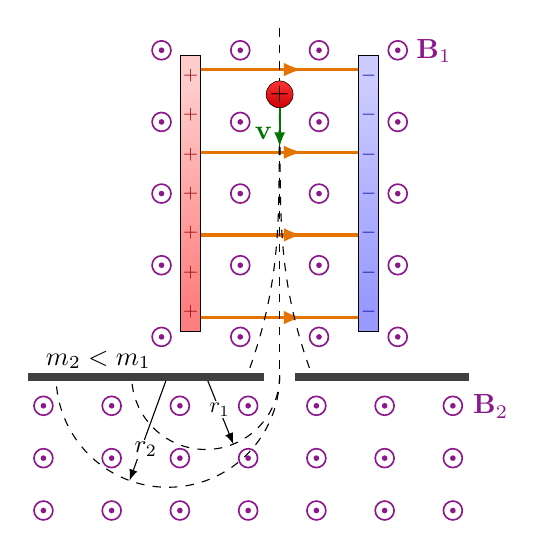
\begin{tikzpicture}
  \def\H{3.5}
  \def\W{2.0}
  \def\w{0.26}
  \def\a{0.15*\W}
  \def\NE{4}
  \def\NQ{7}
  \def\NBx{4}
  \def\NBy{5}
  \def\NBMx{7} % MASS SELECTOR
  \def\NBMy{3}
  
  % ELECTRIC FIELD
  \foreach \i [evaluate={\y=0.05*\H+(\i-1)*(0.9*\H)/(\NE-1);}] in {1,...,\NE}{
    \draw[EFieldLine={0.64},very thick] (0,\y) --++ (\W,0);
  }
  
  % MAGNETIC FIELDS
  \foreach \i [evaluate={\y=-0.02*\H+(\i-1)*(1.04*\H)/(\NBy-1);}] in {1,...,\NBy}{
    \foreach \j [evaluate={\x=-0.25*\W+(\j-1)*(1.5*\W)/(\NBx-1);}] in {1,...,\NBx}{
      \pic[rotate=-90] at (\x,\y) {Bout};
    }
  }
  \foreach \i [evaluate={\y=-0.27*\H-(\i-1)*(0.38*\H)/(\NBMy-1);}] in {1,...,\NBMy}{
    \foreach \j [evaluate={\x=-1.0*\W+(\j-1)*(2.6*\W)/(\NBMx-1);}] in {1,...,\NBMx}{
      \pic[rotate=-90] at (\x,\y) {Bout};
    }
  }
  \node[Bcol,above] at (1.48*\W,0.94*\H) {$\vb{B}_1$};
  \node[Bcol,above] at (1.84*\W,-0.35*\H) {$\vb{B}_2$};
  
  % PLATES
  \draw[anode]
    (0,0) rectangle++ (-\w,\H);
  \draw[cathode]
    (\W,0) rectangle++ (\w,\H);
  \foreach \i [evaluate={\y=(\i-0.5)*\H/\NQ;}] in {1,...,\NQ}{
    \node[pluscol,scale=0.7] at (-\w/2,\y) {$+$};
    \node[minuscol,scale=0.7] at (\W+\w/2,\y) {$-$};
  }
  
  % PARTICLE in capacitor
  \draw[dashed] (\W/2,1.10*\H) --++ (0,-1.26*\H) coordinate (P);
  \draw[dashed] (\W/2,0.85*\H) to[out=-91,in=70] (0.3*\W,-0.15*\H);
  \draw[dashed] (\W/2,0.85*\H) to[out=-89,in=110] (0.7*\W,-0.15*\H);
  %\draw[vector] (P) --++ (0,-0.19*\H) node[above left=-1] {$\vb{v}$};
  
  % PARTICLE in spectrometer
  \draw[dashed] (P) arc (0:-180:{0.47*\W});
  \draw[dashed] (P) arc (0:-180:{0.71*\W}) node[left=6,above right=-1,scale=0.95] {$m_2 < m_1$};
  \node[charge+,scale=0.9] (Q) at (\W/2,0.86*\H) {$+$};
  \draw[vector] (Q) --++ (0,-0.19*\H) node[above left=-1] {$\vb{v}$};
  \draw[->,thin]
    (P)++(-0.47*\W,0) --++ (-68:{0.47*\W})
    node[midway,fill=white,scale=0.8,inner sep=0.9] {$r_1$};
  \draw[->,thin]
    (P)++(-0.71*\W,0) --++ (-110:{0.71*\W})
    node[midway,left=1,below=4,fill=white,scale=0.9,inner sep=0.9] {$r_2$};
  
  
  % SELECTOR WALL
  \fill[black!75]
    (0.4*\W,-0.15*\H) rectangle++ (-1.5*\W,-0.4*\w);
  \fill[black!75]
    (0.6*\W,-0.15*\H) rectangle++ (1.1*\W,-0.4*\w);
  
\end{tikzpicture}



\end{document}